\section{Boundary modes under a physical gate}
\label{sec:boundary-mode}

The authors of \cite{arxiv2601_16277} report that with D1 the $\mnu$ posterior is pushed against the prior border at $\mnu=0$. This section asks, in the simplest possible model, when such boundary behavior arises and how it responds to tightening. Every proposition below is proved in Lean~4 with Mathlib. Appendix~\ref{app:formal} maps each statement to its formal counterpart. The model assumes exactly Gaussian, independent constraints and, for posterior statements, a prior that is constant on the allowed region. These are assumptions of the model, and we have not shown that real CMB or BAO likelihoods satisfy them.

\subsection{Two Gaussian constraints and a gate}
Let $m\ge0$ stand for $\mnu$. Two independent constraints contribute Gaussian factors $\exp[-(m-\mu_i)^2/(2\sigma_i^2)]$ with $\sigma_i>0$ and precisions $a=\sigma_1^{-2}$, $b=\sigma_2^{-2}$. Completing the square gives
\begin{equation}
  a(m-\mu_1)^2+b(m-\mu_2)^2 \;=\; (a+b)(m-\mu_\star)^2+\frac{ab}{a+b}(\mu_1-\mu_2)^2,
  \qquad
  \mu_\star=\frac{a\mu_1+b\mu_2}{a+b},\quad \sigma_\star^2=\frac{1}{a+b}.
  \label{eq:toy_combined_gaussian}
\end{equation}

\begin{proposition}[Gated mode]\label{prop:mode}
On $[0,\infty)$ the product of the two factors has the unique maximizer
\begin{equation}
  m_{\mathrm{mode}}=\max(0,\mu_\star).
  \label{eq:toy_trunc_mode}
\end{equation}
The mode is at the boundary exactly when $a\mu_1+b\mu_2\le0$. In particular, if $\mu_1\ge0$ and $\mu_2\ge0$ then $\mu_\star\ge0$. Multiplying both precisions by the same positive constant leaves $\mu_\star$ unchanged.
\end{proposition}

The second statement is the key qualitative point. Tension between two constraints that both prefer positive masses can never move the mode to zero. A boundary mode needs a nonpositive combined mean. Apart from the edge case in which both means are exactly zero, this requires at least one constraint whose effective mean is negative, a pull towards ``negative mass''. The gate turns this pull into a mode at zero, without negative masses ever being physical (\cref{fig:toy}a).

\begin{proposition}[The gated law]\label{prop:law}
Let $\sigma>0$ and $\mu\in\mathbb{R}$. The kernel $\exp[-(m-\mu)^2/(2\sigma^2)]$ restricted to $m\ge0$ has integral $Z=\sigma\sqrt{2\pi}\,\Phi(\mu/\sigma)>0$, where $\Phi$ is the standard normal CDF. The normalized law is the Gaussian $\mathcal N(\mu,\sigma^2)$ restricted to $[0,\infty)$ and divided by $\Phi(\mu/\sigma)$. Its CDF is
\begin{equation}
  F(x)=\frac{\Phi\!\left(\frac{x-\mu}{\sigma}\right)-\Phi\!\left(-\frac{\mu}{\sigma}\right)}{\Phi\!\left(\frac{\mu}{\sigma}\right)}\quad(x\ge0),\qquad F(x)=0\quad(x\le0),
  \label{eq:gated_cdf}
\end{equation}
which is continuous and strictly increasing on $[0,\infty)$. The law gives zero probability to the point $m=0$ and positive probability to every interval $(0,\varepsilon]$ with $\varepsilon>0$. For every $0<q<1$ it has exactly one $q$-quantile, and that quantile is positive.
\end{proposition}

Thus a density mode at zero is not a probability atom at zero, and upper limits remain well defined and strictly positive. Three quantities should be kept apart: the location of the density mode, the posterior mass in a small interval near zero, and the probability of obtaining a boundary mode across repeated experiments.

\subsection{How tightening changes the chance of a boundary mode}
Suppose the second constraint's mean scatters around the first: $\mu_2=\mu_1+\epsilon$ with offset $\epsilon\sim\mathcal N(-d,s^2)$ and $s>0$. A positive $d$ means that the second constraint tends to prefer smaller masses.

\begin{proposition}[Boundary probability]\label{prop:sweep}
The gated mode is at zero exactly when $\epsilon\le-\mu_1\left(1+\sigma_2^2/\sigma_1^2\right)$, so
\begin{equation}
  P(\mathrm{mode}=0)=\Phi\!\left(\frac{d-\mu_1\left(1+\sigma_2^2/\sigma_1^2\right)}{s}\right).
  \label{eq:sweep_probability}
\end{equation}
Hold $\mu_1$, $\sigma_1$, $d$ and $s$ fixed. If $\mu_1>0$, the probability strictly increases as the second constraint tightens ($\sigma_2$ decreases). If $\mu_1<0$, it strictly decreases. If $\mu_1=0$, it does not depend on $\sigma_2$. Tightening both constraints by a common factor leaves the boundary event unchanged.
\end{proposition}

So ``tighter data make boundary modes more common'' holds only in a specific regime: one constraint is tightened, and the other has a positive mean. It is not a general law (\cref{fig:toy}b). The tightening statement also assumes that the offset distribution stays the same while $\sigma_2$ changes. If a new data release changes both the width and the mean of a constraint, as a lens swap may, the proposition does not apply directly.

\begin{figure}[t]
  \centering
  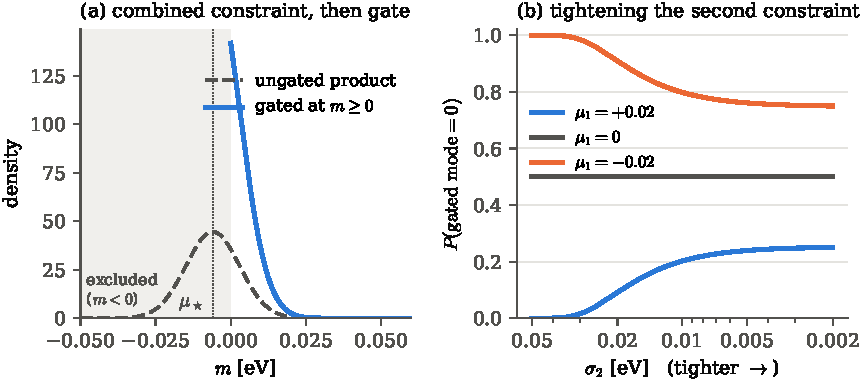
\includegraphics[width=\linewidth]{figures/fig_toy_boundary.pdf}
  \caption{The two-constraint model. (a) With $\mu_1=0.05$, $\sigma_1=0.02$, $\mu_2=-0.02$ and $\sigma_2=0.01$\,eV, the ungated product (dashed) peaks at $\mu_\star=-0.006$\,eV. After the gate, the density (solid) has its mode at $m=0$ but no atom there. (b) Probability of a boundary mode, \cref{eq:sweep_probability}, as the second constraint tightens, for $\mu_1\in\{+0.02,0,-0.02\}$\,eV, $\sigma_1=0.02$\,eV, $d=0$ and $s=0.03$\,eV. Tightening raises the probability when $\mu_1>0$, lowers it when $\mu_1<0$, and leaves it unchanged when $\mu_1=0$.}
  \label{fig:toy}
\end{figure}

\subsection{The finite upper prior and the reading of upper limits}
Posteriors are computed with a finite prior box, here $\mnu\le5$\,eV. The next statement shows what such a box can and cannot hide.

\begin{proposition}[Finite upper gate]\label{prop:upper-gate}
Let $\nu$ be any probability law on $\mathbb{R}$ with CDF $F$ and $F(U)>0$. Conditioning on $m\le U$ gives the CDF $F_U(x)=F(\min(x,U))/F(U)$. For every $x$,
\[
  0\;\le\; F_U(x)-F(x)\;\le\; 1-F(U),
\]
with equality on the right at $x=U$. For the gated Gaussian of \cref{prop:law} and any $U>0$, each level $0<q<1$ has a unique conditioned quantile in $(0,U)$.
\end{proposition}

The error introduced by a finite upper gate is therefore bounded by the probability that the wider posterior assigns above $U$. That probability has to be established separately. A small conditional upper limit does not establish it. As an exact example, take a likelihood equal to $47/10$ on $[0,1/5]$, $3/50$ on $[5,6]$, and zero elsewhere. With a flat prior on $[0,5]$ its 95th percentile is $0.19$\,eV, while with a flat prior on $[0,6]$ it is $31/6\approx5.17$\,eV. We do not suggest that the real likelihood behaves like this. The example only shows why the absence of samples near $5$\,eV is not, by itself, a proof that the prior box is irrelevant.

\begin{proposition}[Comparing two upper limits]\label{prop:readout}
Let $q_A,q_B$ be two upper limits and $\hat q_A,\hat q_B$ their estimates, with $|\hat q_A-q_A|\le\varepsilon_A$ and $|\hat q_B-q_B|\le\varepsilon_B$. Then $|(\hat q_A-\hat q_B)-(q_A-q_B)|\le\varepsilon_A+\varepsilon_B$, and the bound can be attained. If $\hat q_A-\hat q_B>\varepsilon_A+\varepsilon_B$ then $q_A>q_B$. When the estimates are random variables on a common probability space, the probability that the combined bound fails is at most the sum of the two individual failure probabilities, whatever the dependence between the estimates.
\end{proposition}

\subsection{What the model does and does not say about the lens swap}
The model shows that a hard gate can turn a nonpositive combined mean, for example from a moderate negative pull, into a mode at exactly zero, and that whether tightening favors this depends on the sign of the other constraint. It does not show that the SPT lens swap creates such a pull. Nor does it show that the real posteriors are Gaussian or that their constraints are independent. Our own sampled posteriors cannot settle the question (\cref{sec:results-mnu}). The model's practical lesson is about reporting. When the posterior sits against the gate, quantiles of the gated law (\cref{prop:law}) remain meaningful. The location of the mode, in contrast, can switch to or away from zero under modest changes in a constraint's mean.
